%!TEX root = ../dissertation.tex

\chapter{Introduction}
\label{introduction}


\section{Motivation}
\label{cha1:motivation}
Even after years of research, the brain remains to this day a mysterious information-processing biological system. For example, from many of its puzzling abilities, it is still not completely understood how the brain determines which muscles to control in order to fulfill a particular movement task. This task could be something as simple as grasping an object, or even before that, looking at (and identifying) that  object.

The required number of degrees	 of freedom to perform a particular movement is typically much smaller than the ones made available by the muscular apparatus, thus yielding a redundant control problem with infinitely many possibilities. This aspect of motor control has become known as the "Degrees of Freedom Problem" (DOF)\footnote{N. Bernstein, “The Coordination and Regulation of Movements. Oxford : Pergamon Press,” 1967.}, and was first articulated by Nikolai Bernstein in its current form. For example, the eye has six extra-ocular muscles (6 DOF), but to point the eye in any given direction, only two coordinates are needed (the azimuth and the elevation angles). Bernstein theorized that the brain gradually tries to find the optimal control solution for a certain task, to constrain the DOF to the required motor space, which would result in consistent performance. Indeed, when different subjects perform the same task, their muscular activations are remarkably similar. As it will be seen below, the eye orientation thus appears to be constrained by the so-called Donders' law.

Moreover, navigating through an environment in which multiple  stimuli compete for attention, and being equipped with multiple sensory and motor systems to do so, severely complicates the challenges for the brain to rapidly select the optimal plan for a response to achieve a particular goal \cite{johnpage}. This leads to several questions: How does the normal brain decide which signals are "goals", and which are "distractors" in those complex environments? How is the plan to reach the goal truly defined? And how does this differ for sensory-impaired brains? 

When focusing on audiovisual stimuli, it is important to apply the scientifically acquired concepts from neuroscience and psychophysics to an approximate model of the human sensory-motor system (eyes, head, and ears), which is the main topic of this research project.
The idea is to create an autonomous humanoid eye-head robot with foveal vision, realistic auditory inputs, three-dimensional nested eye and head motor systems, and rapid sensory-motor feedback controls and learning algorithms. So far, a working mechanical model of a biologically inspired eye with six muscles has been built in a previous project \cite{tesemiguel}, and is shown in Figure \ref{cha1:sec1:fig:curr_eye_model}.  

This model was constructed with Donders' and Listing's Laws in mind. Donders' law states that the 3D orientation of the eye, when looking in a specific direction, is always the same. Listing propounded that the law could be further constrained by the discovery that the rotation axes corresponding to all possible eye orientations  all lie in a common plane, called Listing's plane. The component of the rotation axis normal to this plane quantifies the eye's torsional orientation component, and results to be close to zero in these conditions. The normal to Listing’s Plane is directed into the so-called \textit{primary direction}, and points about 15 to 30 degrees upwards relative to the straight-ahead viewing direction (head fixed). It is still not well understood which aspects of the ocular motor system determine the primary orientation (and hence, Listing's law).

Whether the rotation axis of eye orientation is programmed by the brain, fully determined by the mechanical properties of the eye muscles, or by both factors, is still not known for sure, and is highly debated in the literature. Yet, implementing this system in a humanoid robot might help at understanding this problem better. Note that for active eye-head movements, for vergence eye movements (near viewing), for vestibular eye movements (head rotations), and for eye-movements under tilted head orientations, Listing’s law no longer holds true, which provides a strong counter argument against the eye muscle (pulley) hypothesis. \cite{donders}

The current prototype uses an \acrfull{imu} to estimate the eye's orientation. Although \acrshort{imu} units are good on acceleration and velocity measurements, they tend to have a significant position drift when determining the orientation, as seen in figure \ref{cha1:sec1:fig:imu}), which is of course a considerable problem when the eye's orientation needs to be established with better than 0.5 deg resolution. Therefore, this project's focus is to study the addition of a camera to the system, in order to determine the orientation of the eye in a more reliable manner for this model. This will hopefully contribute to a better understanding of the eye's control system, and consequently help at restoring impaired vision, which was, after all, Franciscus Donders' ultimate desire.

\begin{figure}[ht]
	\centering
	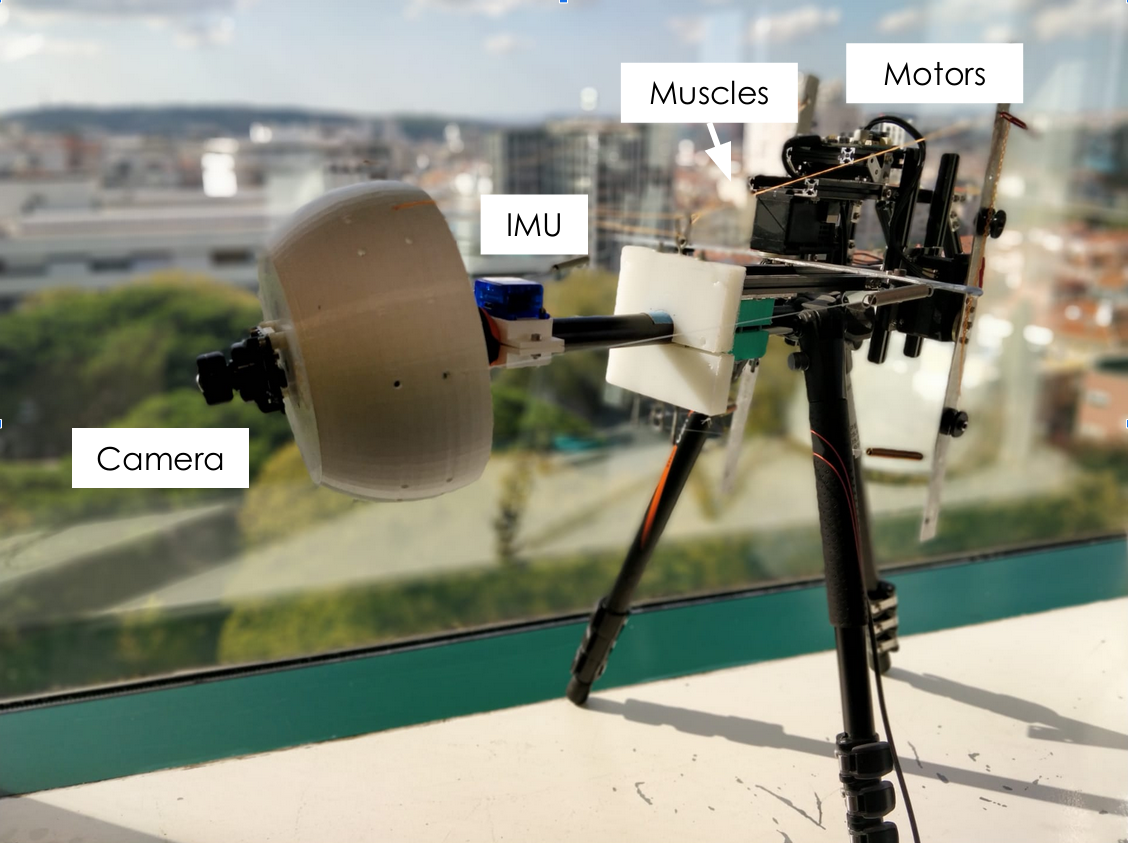
\includegraphics[width=10cm]{images/prototypenew.png}
	\caption[Current mechanical eye model]{The current mechanical eye model. It is composed of an  \acrshort{imu}, seen on the left, and connected to a supportive white eye mounted on a global joint, in turn connected to six elastics, representing the eye muscles, and finally controlled by three motors that pull at those elastics (paired by the aluminum strips). The three motors are controlled by the computer.}
	\label{cha1:sec1:fig:curr_eye_model}
\end{figure}

\begin{figure}[ht]
	\centering
	\begin{minipage}[b]{0.3\linewidth}
		\centering
		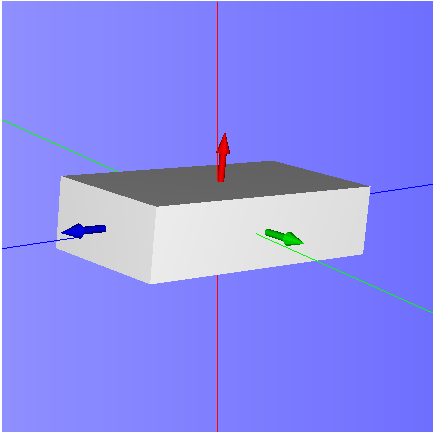
\includegraphics[width=\textwidth]{images/drift1.png}
	\end{minipage}
	\hspace{0.5cm}
	\begin{minipage}[b]{0.3\linewidth}
		\centering
		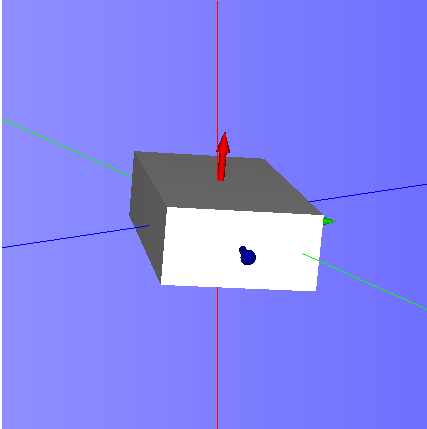
\includegraphics[width=\textwidth]{images/drift2.png}
	\end{minipage}
	\hspace{0.5cm}
	\begin{minipage}[b]{0.3\linewidth}
		\centering
		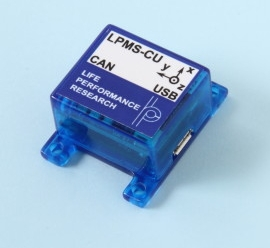
\includegraphics[width=\textwidth]{images/lpmscu.jpg}
	\end{minipage}
	\caption[ \acrshort{imu} sensor's drift]{ \acrshort{imu} sensor's drift. The two images on the left represent the  \acrshort{imu} position on 3D space, between them it can be observed that, in 80 seconds, the  \acrshort{imu} drifts about 60 degrees around the torsional axis. The coordinate system of the  \acrshort{imu} is defined on the image on the right, where the axis in red is the torsional component, z, green is y, and blue is x.}
	\label{cha1:sec1:fig:imu}
\end{figure}

\section{Problem definition}
\label{cha1:problemdef}
As the eye model will eventually rely on accurate camera output, and to foster solid neuroscientifically inspired study with this model, it's indispensable to have the best possible estimates of the camera's orientation. As well as that, the computational speed versus accuracy trade off will also have to be dealt with. The objective of this study is to approximate the current model to a biological eye as well as possible. Thus, determining the instantaneous orientation of the eye in 3D when the gaze direction changes suddenly, which happens, for example, during rapid saccadic eye movements, should be calculated at the appropriate speed.

The accuracy and computational time mainly depend on the complexity of detecting correspondences between consequent images and on the algorithm responsible for calculating the camera's orientation difference between those images. The latter being the focus of this thesis.

There is a long literature on what are the best algorithms to do so. However, the current prototype, seen on figure \ref{cha1:sec1:fig:imu}, has a particularity. There is a translation movement associated to the camera movement that may be defined as a function of the rotation and the fixed length of the camera’s support. To that length, we call baseline and is observable on the left of figure \ref{cha1:sec1:fig:baseline}, as is its effect on the right.

\begin{figure}[ht]
	\centering
	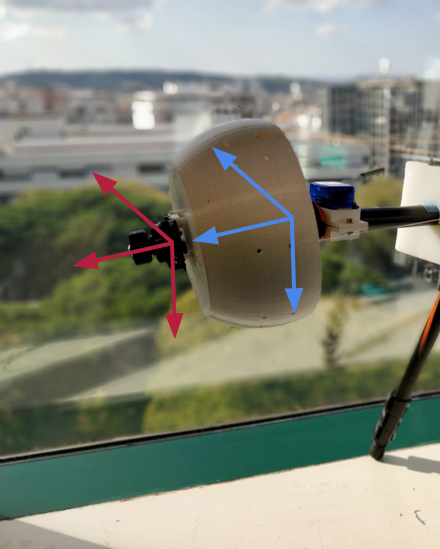
\includegraphics[width=0.4\textwidth]{images/prototypeaxis.png}
	\caption[Baseline associated]{Baseline associated. It shows where the camera's center is, red coordinate system, versus where the eye's rotation center is, blue coordinate system, hence creating a baseline length on the Z coordinate.}
	\label{cha1:sec1:fig:baseline}
\end{figure}

Besides this, there is also another condition to the system. There is no depth information provided because the camera is only \acrshort{rgb}. Hence, the problem is finding the best algorithm to estimate the orientation of a RGB camera with a baseline length associated to the rotational movement.

\section{Objectives}
\label{cha1:objectives}

As mentioned until now, the main objective of this thesis is to develop an algorithm to determine the orientation of the camera in its particular context that works as accurately and fast as possible. Beyond that, this work also aims to:

\begin{itemize}
\item Determine how much accuracy may be gained from using the baseline constraint versus the usual approach;
\item Understand how different algorithms behave in the real world;
\item And evaluate the improvement of using the camera over the  \acrshort{imu}.
\end{itemize}

 		
\section{Outline}
\label{cha1:outline}

The next chapters of this document are structured as follows.
\begin{itemize}
\item	Chapter 2 gives insight on essential concepts necessary to understand this work, along with an overview of the state of the art on the thesis' topic.
	
\item	Chapter 3 explains the methodology used to accomplish the objectives. It describes a novel algorithm to obtain the camera's orientation, how state of the art algorithms were implemented and how all of them were compared against each other. 
	
\item	Chapter 4 presents the results gathered from comparing various estimation algorithms between each other, and with the \acrshort{imu}.
	
\item	Chapter 5 draws conclusions on which algorithm is best to use on the current prototype according to their behavior on the real world. Enlightens the reader on how this work attempts to contribute to science and on future work that shall be done.
	
\end{itemize}



